
\section{ \textbf{Hugo Junkers}}

dsa

\subsection{Biografia}

podsekcja

\begin{frame}{\textbf{Hugo Junkers - Biografia}}
\textbf{Hugo Junkers} urodził się w 1859 roku w rodzinie młynarza i od najmłodszych lat wykazywał zdolności naukowe. Po studiach w Charlottenburgu i Aachen, w 1890 roku rozpoczął pracę w Continental Gas-Gesellschaft w Dessau, gdzie asystował przy pracach nad silnikami spalinowymi. Jego zainteresowanie technologią gazową doprowadziło do pomysłu na piecyk gazowy.
W 1895 roku Junkers opatentował nowoczesny piecyk, który dzięki systemowi podgrzewanych rurek efektywnie podgrzewał wodę, co znacznie zmniejszało zużycie gazu. Jego firma, Junkers \& Co., szybko zyskała popularność, sprzedając 100 tysięcy pieców w ciągu pierwszych piętnastu lat. Jego wynalazek stał się synonimem komfortu w codziennym życiu, przyczyniając się do wzrostu zapotrzebowania na gaz.
\end{frame}

\begin{frame}{\textbf{Hugo Junkers - Biografia}}
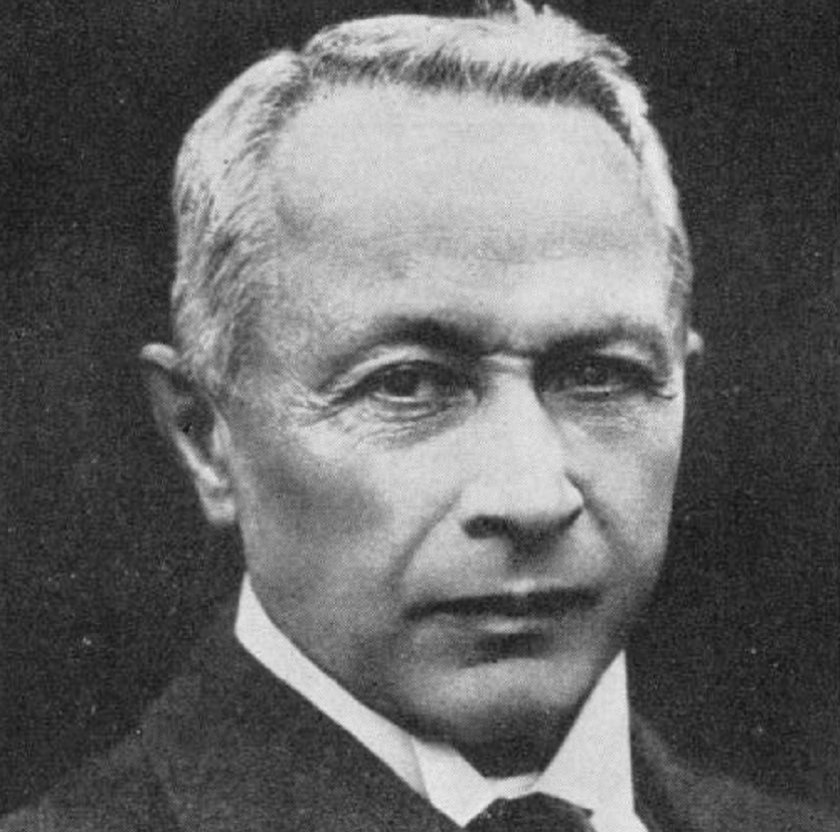
\includegraphics[width=8cm]{images/hugo-01.jpg}
\end{frame}

\begin{frame}{\textbf{Hugo Junkers - Biografia}}
Junkers był także pasjonatem blachy, co zaowocowało wieloma innowacjami, w tym pierwszym całkowicie metalowym samolocie – Junkers J 1 – w 1915 roku. Mimo że był zbyt ciężki, jego konstrukcja wyznaczyła nowy kierunek w lotnictwie. Junkers uruchomił także fabrykę silników lotniczych, a jego najsłynniejszym samolotem pasażerskim stał się Ju-52, zdolny do lotów nad Alpami.
Jednak po dojściu nazistów do władzy, Junkers, będący pacyfistą, odmówił współpracy z reżimem, co doprowadziło do utraty wpływu na swoje przedsiębiorstwa. Fabryki zostały znacjonalizowane i zaczęły produkować samoloty wojskowe, w tym słynne bombowce Junkers-87, używane podczas II wojny światowej.
Hugo Junkers zmarł w 1935 roku w areszcie domowym, nie zdając sobie sprawy z dalszych losów jego firmy. Choć samoloty wojskowe są dziś dostępne tylko w muzeach, jego piecyki gazowe nadal ogrzewają domy na całym świecie, przypominając o jego innowacyjności i wpływie na codzienne życie.
\end{frame}


\begin{frame}{\textbf{Hugo Junkers - Biografia}}
	\begin{center}
		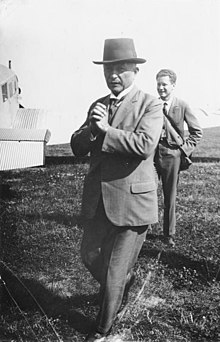
\includegraphics[width=4cm]{images/hugo-02.jpg}
		\caption{My first figure in beamer.}
	\end{center}
\end{frame}